\documentclass[conference]{IEEEtran}
% \IEEEoverridecommandlockouts  % only needed for a funding footnote; none here
\usepackage{cite}
\usepackage{amsmath,amssymb,amsfonts}
\usepackage{graphicx}
\usepackage{textcomp}
\usepackage{booktabs}
% No character protrusion: it pushes line-end punctuation into the column gutter,
% which EDAS measures (minimum 0.12 in).
\usepackage[protrusion=false]{microtype}
\usepackage{tikz}
\usetikzlibrary{arrows.meta,positioning}

\graphicspath{{figures/}}

% ICEE 2026 requires 9 pt captions; IEEEtran sets them in 8 pt (\footnotesize).
% This is IEEEtran's conference \@makecaption with \small (9 pt) in its place.
\makeatletter
\long\def\@makecaption#1#2{%
\ifx\@captype\@IEEEtablestring%
\small\bgroup\par\centering\@IEEEtabletopskipstrut{\normalfont\small #1}\\%
{\normalfont\small\scshape #2}\par\addvspace{0.5\baselineskip}\egroup%
\@IEEEtablecaptionsepspace
\else
\@IEEEfigurecaptionsepspace
\setbox\@tempboxa\hbox{\normalfont\small {#1.}\nobreakspace\nobreakspace #2}%
\ifdim \wd\@tempboxa >\hsize%
\setbox\@tempboxa\hbox{\normalfont\small {#1.}\nobreakspace\nobreakspace}%
\parbox[t]{\hsize}{\normalfont\small\noindent\unhbox\@tempboxa#2}%
\else%
\hbox to\hsize{\normalfont\small\hfil\box\@tempboxa\hfil}%
\fi\fi}
\makeatother
\newcommand{\SN}{R}            % signal-to-noise power ratio, S/N
\newcommand{\dB}{~dB}

\begin{document}

\title{Feed-Forward Spiking Networks Obey a Friis-Type Cascade Law: Fidelity
Ceilings and a Fan-In Design Rule for Biosignal Processing}

\author{\IEEEauthorblockN{Ahad Ulla Baig}
\IEEEauthorblockA{\textit{Dept. of Artificial Intelligence} \\
\textit{and Machine Learning} \\
\textit{Ramaiah Institute of Technology}\\
Bengaluru, India \\
ahadullabaig.16@gmail.com}
\and
\IEEEauthorblockN{Divisha Gera}
\IEEEauthorblockA{\textit{Dept. of Artificial Intelligence} \\
\textit{and Machine Learning} \\
\textit{Ramaiah Institute of Technology}\\
Bengaluru, India \\
divisha.018@gmail.com}
\and
\IEEEauthorblockN{Charithra G}
\IEEEauthorblockA{\textit{Dept. of Artificial Intelligence} \\
\textit{and Machine Learning} \\
\textit{Ramaiah Institute of Technology}\\
Bengaluru, India \\
charithra754@gmail.com}
}

\maketitle

\begin{abstract}
Spiking neural networks promise always-on biosignal processing on neuromorphic
hardware, but how faithfully they reproduce an analog signal is rarely
quantified. We show that feed-forward leaky integrate-and-fire networks have a
fidelity ceiling. On 16 MIT-BIH ECG records and three synthetic signals, output
SNR rises by less than 0.1 dB per dB of input SNR above 10 dB, and the ceiling
persists under time-to-first-spike and delta coding. An inverse-SNR cascade
law with the form of Friis's noise formula predicts the output on real ECG to
within 0.04 dB RMS over a 60 dB input range, with no fitted parameters. The
ceiling is set by noise that neurons share: wider populations and causal
readout windows do not raise it, and unsupervised STDP lowers it while
collapsing effective fan-in from 24 inputs to about 3. A fixed fan-in of 16
raises it by 1.85 dB over dense connectivity of the same width, to 5.77 dB, the
highest ECG ceiling we measured, with 32 times fewer synapses. A standard ECG
filter still recovers heartbeats better than any configuration tested, so
these are limits and design rules for neuromorphic signal chains, not a new
denoiser.
\end{abstract}

\begin{IEEEkeywords}
spiking neural networks, neuromorphic computing, signal reconstruction,
ECG, noise cascade, sparse connectivity
\end{IEEEkeywords}

\section{Introduction}

Neuromorphic processors run spiking neural networks (SNNs) with sparse,
event-driven computation~\cite{davies2018loihi}, which suits always-on
biosignal processing at the sensor. A recent review finds that most SNN
studies of the electrocardiogram (ECG) target arrhythmia detection, a
classification task~\cite{choi2024biomedical}. SNNs that return a continuous
signal are trained with supervision and avoid spike-rate coding at the input,
the output or both~\cite{ren2026dcpa,henkes2024regression}. Rate coding is
known to be lossy: in an image-denoising study a rate-coded SNN scored almost
8~dB below the other spiking variants~\cite{castagnetti2023spiden}. Theory
shows that noise shared across neurons limits the information a population
carries~\cite{morenobote2014information,kanitscheider2015origin}, but we are
not aware of work that uses it to predict or design the fidelity of spiking
signal chains.

When a rate-calibrated network of leaky integrate-and-fire (LIF) neurons
reconstructs a noisy ECG, raising the input signal-to-noise ratio (SNR) from 20
to 40\dB{}, a hundredfold cut in noise power, lifts the output by about
0.1\dB. We call this plateau the \emph{fidelity ceiling}. The network is not a
competitive denoiser (Section~\ref{sec:discussion}), so we treat the ceiling as
a limit of such signal chains and ask what sets it. Our contributions are:
\begin{itemize}
\item \emph{The ceiling} is flat in input SNR on real and synthetic ECG, a
synthetic electroencephalogram (EEG) and a sine, under three spike codes.
Width, causal readout windows and spike-timing-dependent plasticity (STDP) do
not raise it (Sections~\ref{sec:flat},~\ref{sec:levers}).
\item \emph{A cascade law} of Friis's form predicts output SNR on real ECG to
within 0.04\dB{} RMS over a 60\dB{} input range with no fitted parameters
(Sections~\ref{sec:law},~\ref{sec:flat}).
\item \emph{A mechanism and a design rule.} The binding noise is shared across
neurons. A fixed fan-in of 8--16 raises the ceiling by up to 1.85\dB{} with
16--32 times fewer synapses; STDP lowers it by collapsing fan-in
(Section~\ref{sec:mechanism}).
\end{itemize}

\section{Pipeline and Measurement}
\label{sec:methods}

\subsection{Network}
A scalar signal sampled at 250~Hz (time step 4~ms) is copied to 32 Poisson
encoders, each firing with probability proportional to the amplitude
normalized to the drive's own minimum and maximum. Two all-to-all layers of 16
and 8 LIF neurons follow (the network $[32,16,8]$ of Fig.~\ref{fig:pipeline};
rest $-70$~mV, threshold $-55$~mV, reset $-80$~mV, membrane time constant 20~ms, refractory period 2~ms), with nonnegative weights drawn
uniformly from $[0, 0.3]$. The output is the mean of the output neurons'
exponentially filtered spike trains (time constant 20~ms), a causal readout.
Where stated, pair-based trace STDP (time constants 20~ms, weights bounded to
$[0,1]$), a form of the plasticity used for label-free SNN
learning~\cite{diehl2015unsupervised}, trains the network on the noisy input.

Output quality depends strongly on firing rate, so we hold rates fixed: the
encoder's maximum rate and each layer's synaptic gain are bisected until the
encoder and every layer fire at 40~Hz on the drive, following established SNN
rate normalization~\cite{diehl2015balancing,rueckauer2017conversion}. Trained
networks are recalibrated after learning, so that only their weights differ.
We also report the network as shipped: weights uniform on $[0,1]$, one global
gain and free rates.

\subsection{Signals}
Real ECG comes from 16 records of the MIT-BIH Arrhythmia
Database~\cite{moody2001impact,goldberger2000physionet}: 100, 101, 103, 105,
108, 112, 113, 119, 200, 207, 212, 214, 228, 231, 232 and 234. Each seed takes a
different artifact-free 10~s window, resampled from 360 to 250~Hz. We
add three 10~s synthetic signals: an ECG at 60~beats/min, an EEG made of 10,
20 and 40~Hz components with random phases, and a 2~Hz sine. Gaussian noise is
scaled so that the input SNR against the clean signal equals its nominal value
exactly; the flatness grid spans $-20$ to $+40$\dB{} in 5\dB{} steps plus a
noiseless input. Each condition runs with 10 seeds.

\subsection{Fidelity metric}
A readout's gain and offset are arbitrary, so we fit $\hat{x} = ay + b$ to the
clean signal $x$ by least squares and score the affine-corrected
$\mathrm{SNR} = \mathrm{var}(x)/\mathrm{var}(x-\hat{x})$, quoted in dB. For a
signal plus independent noise this equals $1/(1-\rho^2) = 1 + \SN$, where
$\rho$ is the correlation and $\SN$ the signal-to-noise power ratio, S/N. The
\emph{ceiling} is the output SNR at noiseless input. Runs with a constant
output, or with half the output neurons at 90\% of the maximum rate or more,
are excluded from SNR averages; only trained shipped networks and networks held
at 0.25~Hz ever were. SNRs are causal unless marked
\emph{delay-compensated}, in which case the output is advanced by its best lag
in 0--64~ms.

\subsection{Statistics}
The unit of analysis is a record ($n = 16$) or, for synthetic signals, a seed
($n = 10$). Paired comparisons use the Wilcoxon signed-rank test with Holm
correction within each family, and report the median difference with a
bias-corrected and accelerated (BCa) bootstrap 95\% interval from 10\,000
resamples. Invariance is claimed only by equivalence (two one-sided tests,
margin $\pm 0.5$\dB{}). Tests and margins for the main comparisons were
written down before their grids ran, and checks added after seeing data are
labeled post hoc. The results draw on more than 65\,000 simulations.

\section{A Cascade Law for Spiking Stages}
\label{sec:law}

\begin{figure}[t]
\centering
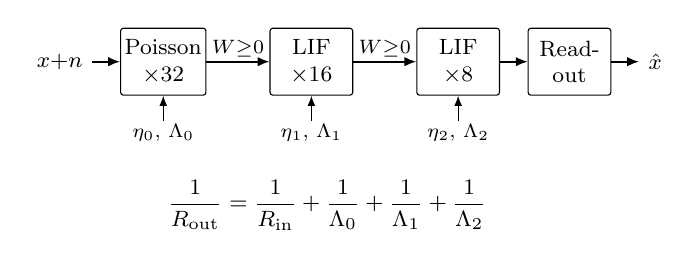
\begin{tikzpicture}[
  font=\footnotesize,
  blk/.style={draw, rounded corners=1pt, minimum height=8.5mm,
    minimum width=10.5mm, align=center, inner sep=1.5pt},
  arr/.style={-{Latex[length=1.5mm,width=1.2mm]}, semithick},
  noise/.style={-{Latex[length=1.3mm,width=1mm]}, thin},
  node distance=8mm]
\node (in) {$x{+}n$};
\node[blk, right=3.5mm of in] (enc) {Poisson\\$\times 32$};
\node[blk, right=of enc] (l1) {LIF\\$\times 16$};
\node[blk, right=of l1] (l2) {LIF\\$\times 8$};
\node[blk, right=3.5mm of l2] (ro) {Read-\\out};
\node[right=3.5mm of ro] (out) {$\hat{x}$};
\draw[arr] (in) -- (enc);
\draw[arr] (enc) -- node[above=1pt, inner sep=0.5pt] {\scriptsize $W{\ge}0$} (l1);
\draw[arr] (l1) -- node[above=1pt, inner sep=0.5pt] {\scriptsize $W{\ge}0$} (l2);
\draw[arr] (l2) -- (ro);
\draw[arr] (ro) -- (out);
\foreach \b/\k in {enc/0, l1/1, l2/2} {
  \node[below=3.2mm of \b, inner sep=1pt] (n\k) {\scriptsize $\eta_\k$, $\Lambda_\k$};
  \draw[noise] (n\k) -- (\b);
}
\node[below=9.5mm of l1, xshift=2mm] {$\dfrac{1}{\SN_\mathrm{out}} =
  \dfrac{1}{\SN_\mathrm{in}} + \dfrac{1}{\Lambda_0} + \dfrac{1}{\Lambda_1}
  + \dfrac{1}{\Lambda_2}$};
\end{tikzpicture}
\caption{The pipeline and its noise model. Each stage adds its own
spike-sampling noise $\eta_k$, so inverse S/N ratios add \eqref{eq:law};
$\Lambda_k$ is the stage's intrinsic S/N.}
\label{fig:pipeline}
\end{figure}

Write stage $k$'s readout as what it inherits plus the noise it adds,
$y_k = G_k\, y_{k-1} + \eta_k$, where $\eta_k$ is the stage's own spike
sampling noise, independent of upstream noise. The gain $G_k$ scales signal
and inherited noise alike and cancels from their ratio, leaving
\begin{equation}
\frac{1}{\SN_k} = \frac{1}{\SN_{k-1}} + \frac{1}{\Lambda_k}, \qquad
\Lambda_k = \frac{G_k^2 S_{k-1}}{\mathrm{var}(\eta_k)},
\label{eq:stage}
\end{equation}
where $S_{k-1}$ is the signal power arriving at the stage and $\Lambda_k$ is
its \emph{intrinsic} S/N. Summing over stages gives
\begin{equation}
\frac{1}{\SN_\mathrm{out}} = \frac{1}{\SN_\mathrm{in}} + \sum_k
\frac{1}{\Lambda_k}, \qquad
C = \Bigl(\sum_k \frac{1}{\Lambda_k}\Bigr)^{-1}.
\label{eq:law}
\end{equation}
It has the form of Friis's cascade formula for the noise figure of amplifier
chains~\cite{friis1944noise}, written in inverse S/N. As $\SN_\mathrm{in} \to \infty$ the
output tends to $C$, the ceiling, which is set by the network alone. Three
predictions follow: output quality stops tracking the input once
$\SN_\mathrm{in} \gg C$; every added stage adds a positive term; and improving
a stage whose $1/\Lambda_k$ is a small part of the sum does little.

Two conditions make \eqref{eq:law} accurate to a few hundredths of a dB on ECG
and EEG. It holds for $\SN$, not
for the affine-corrected $\mathrm{SNR} = 1 + \SN$, which must be converted
before the law is applied, or the law over-predicts loss by about 2\dB{} below
10\dB{} input. And $C$ must be measured at the input's operating point: the
encoder's range and the calibrated gains follow the noisy drive, so for each
input level we measure $C$ with a noiseless run that uses the operating point
that level's noisy drive sets.

\emph{Where $\Lambda$ comes from.} Averaging $N$ neurons whose readout errors
have variance $\sigma_1^2$ and mean pairwise correlation $c$ gives
\begin{equation}
\Lambda(N) = \frac{\sigma_s^2}{\sigma_1^2\,[\,1/N + c\,(1-1/N)\,]}
\;\xrightarrow{N\to\infty}\; \frac{\sigma_s^2}{c\,\sigma_1^2},
\label{eq:width}
\end{equation}
with $\sigma_s^2$ the signal variance in one neuron's trace. Shared error caps
what width can buy, as shared input noise caps population
information~\cite{morenobote2014information}. The noise in two neurons' drives
is correlated through the overlap of their input
filters~\cite{kanitscheider2015origin}; for independent, equal-variance inputs
the correlation is the cosine similarity of their weight columns,
$\mu^2/(\mu^2+\sigma^2)$ for independent, identically distributed weights of
mean $\mu$ and
variance $\sigma^2$. Any uniform draw on $[0,a]$ gives $3/4$ whatever $a$, so
rescaling weights, as rate calibration does, cannot change it. Giving each
neuron fewer inputs lowers the overlap but leaves it fewer spike trains to
average, so fan-in should have an optimum.

\section{Results}

\subsection{The ceiling is flat, and the law predicts it}
\label{sec:flat}

\begin{figure}[t]
\centering
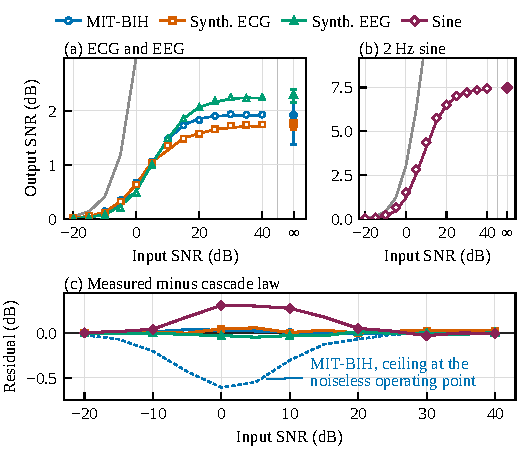
\includegraphics[width=\columnwidth]{fig1_ceiling_law.pdf}
\caption{Rate-controlled network, untrained. (a, b) Output SNR against input
SNR: markers are medians over records or seeds, lines are the cascade
law~\eqref{eq:law} with the ceiling measured at each input's operating point,
the grey line is the unprocessed input, and the $\infty$ column is the
noiseless ceiling with its interquartile range. (c) Measured minus predicted
output SNR; dashed, the law with the ceiling of the ordinary noiseless run.}
\label{fig:ceiling}
\end{figure}

With every layer at 40~Hz, output SNR saturates on all four signals
(Fig.~\ref{fig:ceiling}a, b). Above 10\dB{}, where the input's own SNR rises
0.99\dB{} per dB, the output rises $+0.012$ [$+0.005$, $+0.014$]\dB{} per dB on
MIT-BIH and at most $+0.092$ (sine), and every 95\% interval excludes~1. The
shipped network, untrained or after 10 STDP epochs, is as flat (slopes at most
0.07). The ceiling is 1.92\dB{} on MIT-BIH (interquartile range 1.38--2.27),
1.76 on synthetic ECG, 2.29 on EEG and 7.48 on the sine: flat everywhere, with
a height that depends on the signal.

The law predicts the MIT-BIH output with an RMS residual of 0.02\dB{} at
inputs of 10\dB{} and above and 0.04\dB{} below, and at most 0.11\dB{} over all
208 record-level points (Fig.~\ref{fig:ceiling}c); on synthetic ECG and EEG the
RMS is 0.04--0.07\dB. The sine keeps an unexplained bias of up to $+0.3$\dB{}
between 0 and 10\dB{} input. Without the operating-point match the MIT-BIH
residual below 10\dB{} grows to 0.39\dB{} RMS (dashed). Noise widens the
encoder's range and squeezes the signal into less of it; at 0\dB{} input this
alone costs 1.1\dB{} of ceiling. This check was designed after we saw the
residual of the ordinary form.

\subsection{What moves the ceiling}
\label{sec:levers}

% Generated by scripts/paper_icee2026/figures.py — do not edit.
\begin{table}[t]
\centering
\caption{What Moves the MIT-BIH Ceiling}
\label{tab:levers}
\scriptsize
\setlength{\tabcolsep}{3pt}
\begin{tabular}{@{}lll@{}}
\toprule
Manipulation & Ceiling (dB) & Change (dB) [95\% CI] \\
\midrule
\multicolumn{3}{@{}l}{\emph{Does not raise it}} \\
Output width, 8 to 64 & $1.92\,{\to}\,1.99$ & {\boldmath $+0.08$ [$+0.06$, $+0.09$]} $\equiv$ \\
Readout $\tau$, 20 to 40~ms (best) & $1.92\,{\to}\,1.98$ & $+0.21$ [$-0.06$, $+0.26$] $\equiv$ \\
Time-to-first-spike code & $2.86\,{\to}\,2.28$$^{\mathrm{a}}$ & $-0.76$ [$-1.13$, $+0.24$] \\
\midrule
\multicolumn{3}{@{}l}{\emph{Lowers it}} \\
STDP, 10 epochs & $1.92\,{\to}\,1.34$ & {\boldmath $-0.49$ [$-0.60$, $-0.39$]} \\
STDP, 200 epochs & $1.92\,{\to}\,1.06$ & {\boldmath $-0.64$ [$-0.75$, $-0.56$]} \\
Depth, 3 to 4 layers & $1.92\,{\to}\,1.57$ & {\boldmath $-0.36$ [$-0.40$, $-0.30$]} $\equiv$ \\
Delta code & $2.86\,{\to}\,0.61$$^{\mathrm{a}}$ & {\boldmath $-1.63$ [$-2.25$, $-1.24$]} \\
\midrule
\multicolumn{3}{@{}l}{\emph{Raises it}} \\
Depth, 3 to 2 layers & $1.92\,{\to}\,2.75$ & {\boldmath $+0.91$ [$+0.79$, $+1.09$]} \\
Output rate, 40 to 5~Hz$^{\mathrm{b}}$ & $1.99\,{\to}\,2.71$ & {\boldmath $+0.81$ [$+0.17$, $+1.48$]} \\
Fan-in, all to 16$^{\mathrm{c}}$ & $4.06\,{\to}\,5.77$ & {\boldmath $+1.85$ [$+1.38$, $+2.26$]} \\
\bottomrule
\end{tabular}
\\[2pt]
\parbox{\columnwidth}{\scriptsize Noiseless-input output SNR, median over 16 records; change is the paired median with a BCa interval. Reference: untrained $[32,16,8]$, every layer at 40~Hz, Poisson code, 20~ms exponential readout; STDP rows hold rates. $^{\mathrm{a}}$Delay-compensated SNR against the best Poisson readout (output advanced by its best lag in 0--64~ms). $^{\mathrm{b}}$64 output neurons. $^{\mathrm{c}}$One-layer $[512,512]$ network, both at their best rate (20~Hz). Bold: significant (Wilcoxon signed-rank test, Holm correction within each family). $\equiv$: equivalent within $\pm 0.5$~dB (two one-sided tests).}
\end{table}


Table~\ref{tab:levers} tests each design choice on MIT-BIH.
\emph{Width}: sixteen times the output population buys $+0.08$\dB{}, and every
width from 4 to 64 is equivalent; independent neurons would have gained
$+0.79$\dB{} by~\eqref{eq:width} with $c=0$, and the fitted $c$ is 0.48.
\emph{Readout}: the exponential window has an optimum at 20--40~ms, and windows
of 5, 10 and 160~ms cost 0.75--1.06\dB. \emph{Coding}: a time-to-first-spike
code, read by the population's first-spike latency, does not raise the ceiling
on any of the four signals, even on delay-compensated SNR (equivalent on the
sine, lower but not significantly so elsewhere). With the output at 5~Hz, too
sparse for every neuron to fire in every window, it falls 2.7--5.3\dB{} below
Poisson on three of the four signals. A delta code with its threshold
calibrated to 40~Hz follows $|dx/dt|$ rather than $x$ and scores significantly
lower on both ECGs and the sine. For all three codes, all four signals and both output rates, the output
slope above 10\dB{} stays below 1 (24 of 24 cells).

\emph{Depth and learning} lower the ceiling, as~\eqref{eq:law} requires of
depth: 2, 3 and 4 layers give 2.75, 1.92 and 1.57\dB. Ten STDP epochs with
rates held cost 0.49\dB{} and 200 epochs 0.64\dB. As shipped, training mainly
moves the output rate, from 65~Hz to about 1~Hz. \emph{Output rate} is the
largest operating-point lever. With 64 output neurons at 5~Hz the ceiling is
2.71\dB{} against 1.99 at 40~Hz, while the output layer fires eight times
less. The optimum depends on the signal's bandwidth (post hoc): EEG peaks between 10
and 40~Hz and the sine at 40~Hz.

\subsection{Mechanism: shared error and fan-in}
\label{sec:mechanism}

\begin{figure}[t]
\centering
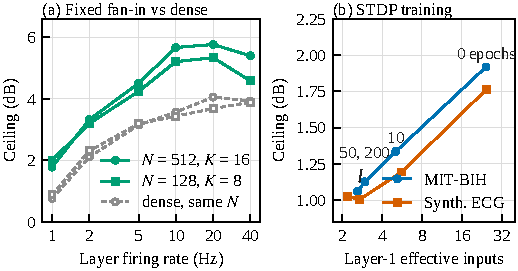
\includegraphics[width=\columnwidth]{fig2_fan_in.pdf}
\caption{Fan-in. (a) MIT-BIH, medians over 16 records: one-layer $[N, N]$
networks held at each firing rate, each neuron drawing exactly $K$ random
inputs (solid) or all $N$ (dashed). (b) Layer-1 effective inputs,
$(\sum_i w_i)^2/\sum_i w_i^2$ per weight column, against the ceiling of the
rate-controlled $[32,16,8]$ network at 0, 10, 50 and 200 STDP epochs; medians
over records (MIT-BIH) or seeds (synthetic ECG).}
\label{fig:fanin}
\end{figure}

We tested the fan-in trade-off in one-layer $[N,N]$ networks whose neurons each
draw exactly $K$ random inputs, so that fan-in and column cosine ($3K/4N$) can
be varied separately. At 40~Hz the ceiling peaks at $K = 8$--16 at every width
from 32 to 512, improving on dense weights in all 16 records, and the error
correlation tracks column cosine ($R^2 = 0.85$). The gain holds at every firing
rate from 1 to 40~Hz (Fig.~\ref{fig:fanin}a; Wilcoxon $p < 10^{-4}$ at each
rate). At each configuration's best rate, $K = 16$ in $[512,512]$ reaches
5.77\dB{}, $+1.85$ [$+1.38$, $+2.26$]\dB{} over dense weights, and $K = 8$ in
$[128,128]$ gains $+1.10$ [$+0.73$, $+1.57$]\dB{}. In S/N terms, 5.77\dB{} is
five times that of the reference $[32,16,8]$ network (2.78 against 0.56). The two sparse
networks use 32 and 16 times fewer synapses than their dense counterparts and,
at the same firing rates, as many times fewer synaptic events.

STDP falls off the other side of the same trade-off. On the tiled input it
depresses most of each layer-1 neuron's synapses: the effective number of
inputs falls from 24.3 to 5.1, 3.0 and 2.6 at 10, 50 and 200 epochs
(Fig.~\ref{fig:fanin}b). Across records and epoch counts the drop tracks the loss of layer-1
intrinsic S/N (Spearman $\rho = +0.79$, $p = 4\times10^{-11}$, $n = 48$),
whereas the change in column cosine does not ($\rho = +0.11$, $p = 0.45$);
training in fact \emph{decorrelates} layer-1 columns (cosine 0.76 to 0.38).
A neuron averaging three Poisson trains is far noisier than one averaging~24.
Dense random weights sit on the high-overlap side of the optimum and trained
weights on the low-fan-in side.

\section{Discussion}
\label{sec:discussion}

\emph{Design rules.} Like a radio-frequency receiver chain, a spiking pipeline
can be budgeted stage by stage: one noiseless run at the operating point gives
each $\Lambda_k$, and \eqref{eq:law} gives the output at any input. For the
class of networks studied here:
\begin{itemize}
\item Once the sensor's S/N is ten times the ceiling, improving it can add at
most 0.4\dB{} of output S/N; change the network instead.
\item Use as few spiking stages as possible: removing one of three layers
gains 0.91\dB.
\item Give each neuron 8--16 inputs, not all of them: up to $+1.85$\dB{} with
16--32 times fewer synapses.
\item Match the output rate to the signal: for ECG a 5~Hz output beats 40~Hz
while firing eight times less; for a sine it does not.
\item Take the encoder's range from a 40~Hz low-pass copy of the input: at
0\dB{} input this adds 0.35\dB{} on MIT-BIH (below the 0.5\dB{} bar we set in
advance) and 1.0\dB{} on the sine, at no cost to the ceiling.
\end{itemize}

\emph{Implications for devices.} Memristive synapses store weights as
conductances, which cannot be negative; signed weights are commonly built from
differential pairs of devices~\cite{prezioso2015training}. Dense, nonnegative,
uniformly random connectivity is exactly the regime in which weight columns
overlap by 3/4. Equation~\eqref{eq:width} suggests two remedies: sparse
fan-in, measured here, and zero-mean signed weights, which remove the overlap
but double the device count and are untested. Whether constraining fan-in
during on-chip learning prevents the loss is also untested.

\emph{Limitations.} All results are simulations of feed-forward LIF networks
without inhibition, recurrence or trained readouts, fed one signal copied
across the input population. When each input channel instead carries its own
noise, width gains only 0.09\dB{} per doubling on MIT-BIH, 2.8\% of what
independent samples allow, so shared input noise does not explain the ceiling.
Every ceiling above is causal; removing the readout's delay offline (post hoc)
raises the best MIT-BIH ceiling from 1.98 to 2.86\dB{} (0.7--4.2\dB{} across
signals), and it stays flat. A signed delta code was not tested. Clinically,
the network does not compete with conventional preprocessing: scored against
the annotations with three QRS detectors in
NeuroKit2~\cite{makowski2021neurokit2}, the noisy input after the toolbox's
standard cleaning filters beats the best network condition significantly in 16
of 18 input and detector combinations, and loses in none.

\section{Conclusion}

Feed-forward spiking networks for biosignal processing have a fidelity ceiling
that is flat in input quality across three spike codes and four signals, and a
Friis-type cascade law predicts their output to within a few hundredths of a dB
on ECG and EEG. The ceiling is set by error that neurons share: width and
learning do not raise it, and a fixed fan-in of 8--16 inputs does, with fewer
synapses.

\bibliographystyle{IEEEtran}
\bibliography{refs}

\end{document}
